\documentclass[compress]{beamer}
\usepackage{ifthen,verbatim}

\newcommand{\isnote}{}
\xdefinecolor{lightyellow}{rgb}{1.,1.,0.25}
\xdefinecolor{darkblue}{rgb}{0.1,0.1,0.7}

%% Uncomment this to get annotations
%% \def\notes{\addtocounter{page}{-1}
%%            \renewcommand{\isnote}{*}
%% 	   \beamertemplateshadingbackground{lightyellow}{white}
%%            \begin{frame}
%%            \frametitle{Notes for the previous page (page \insertpagenumber)}
%%            \itemize}
%% \def\endnotes{\enditemize
%% 	      \end{frame}
%%               \beamertemplateshadingbackground{white}{white}
%%               \renewcommand{\isnote}{}}

%% Uncomment this to not get annotations
\def\notes{\comment}
\def\endnotes{\endcomment}

\setbeamertemplate{navigation symbols}{}
\setbeamertemplate{headline}{\mbox{ } \hfill
\begin{minipage}{5.5 cm}
\vspace{-0.75 cm} \small
\end{minipage} \hfill
\begin{minipage}{4.5 cm}
\vspace{-0.75 cm} \small
\begin{flushright}
\ifthenelse{\equal{\insertpagenumber}{1}}{}{Jim Pivarski \hspace{0.2 cm} \insertpagenumber\isnote/\pageref{numpages}}
\end{flushright}
\end{minipage}\mbox{\hspace{0.2 cm}}\includegraphics[height=1 cm]{../cmslogo} \hspace{0.01 cm} \vspace{-1.05 cm}}

\newcommand{\s}[1]{{\mbox{\scriptsize #1}}}

\begin{document}
\begin{frame}
\vfill
\begin{center}
\textcolor{darkblue}{\Large Quirks: a Rough Trigger Study \\ \vspace{0.2 cm} (to make a trigger choice)}

\vfill
\begin{columns}
\column{0.3\linewidth}
\begin{center}
\large
Jim Pivarski
\end{center}
\end{columns}

%% \begin{columns}
%% \column{0.3\linewidth}
%% \begin{center}
%% \scriptsize
%% {\it Fermilab}
%% \end{center}
%% \end{columns}

\vfill
22 September, 2011

\end{center}
\end{frame}

%% \begin{notes}
%% \item This is the annotated version of my talk.
%% \item If you want the version that I am presenting, download the one
%% labeled ``slides'' on Indico (or just ignore these yellow pages).
%% \item The annotated version is provided for extra detail and a written
%% record of comments that I intend to make orally.
%% \item Yellow notes refer to the content on the {\it previous} page.
%% \item All other slides are identical for the two versions.
%% \end{notes}

\small

\begin{frame}
\frametitle{Reminder}

\hfill 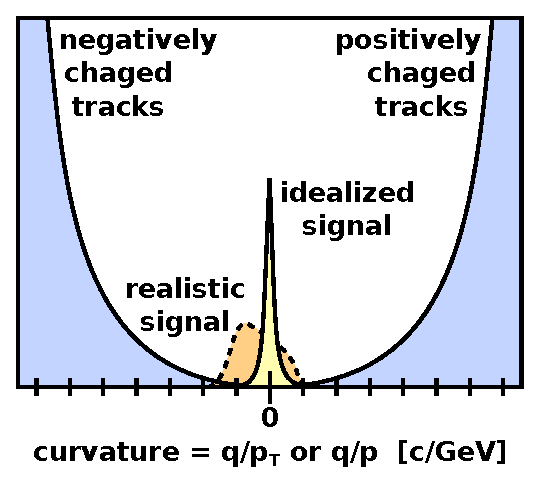
\includegraphics[width=0.3\linewidth]{curvature_distribution.pdf}

\vspace{-3.3 cm}
\begin{itemize}
\item Quirk-pair signature: isolated HSCP with \\ zero curvature
\item Analysis can use $dE/dx$ and $\kappa = q/p_T$ to \\ control backgrounds well \\ (perhaps only modest cuts are needed to \\ eliminate backgrounds)
\item Trigger may be an issue, for the same reason as all HSCP analyses
\end{itemize}

\vspace{0.2 cm}
\hspace{-0.83 cm} \textcolor{darkblue}{\Large This study}
\vspace{0.1 cm}
\begin{itemize}
\item I have received a generator-level ntuple from Jared Evans and Markus Luty \\ {\tiny (100 and 250~GeV/$c^2$ charged, uncolored quirks at 7~TeV, $\Lambda$ is relevant only for reconstruction, \\ \vspace{-0.15 cm} $SU(N)$ where $N=2$, but cross-section is simply proportional to $N$)}
\item I have a muon trigger vs.\ $\beta$ curve from Chris Farrell
\item Checked current trigger thresholds and prescales on ConfDB
\item \textcolor{darkblue}{Goal:} choose an appropriate trigger/set of triggers
\end{itemize}
\end{frame}

\begin{frame}
\frametitle{Muon trigger vs.\ $\beta$ curve}
\framesubtitle{Note that \textcolor{red}{GlobalMuon-plus-trigger match (red)} is nearly flat in $\eta$ and flat at high $p_T$ \\ Only significant dependence is on $\beta$}

\begin{center}
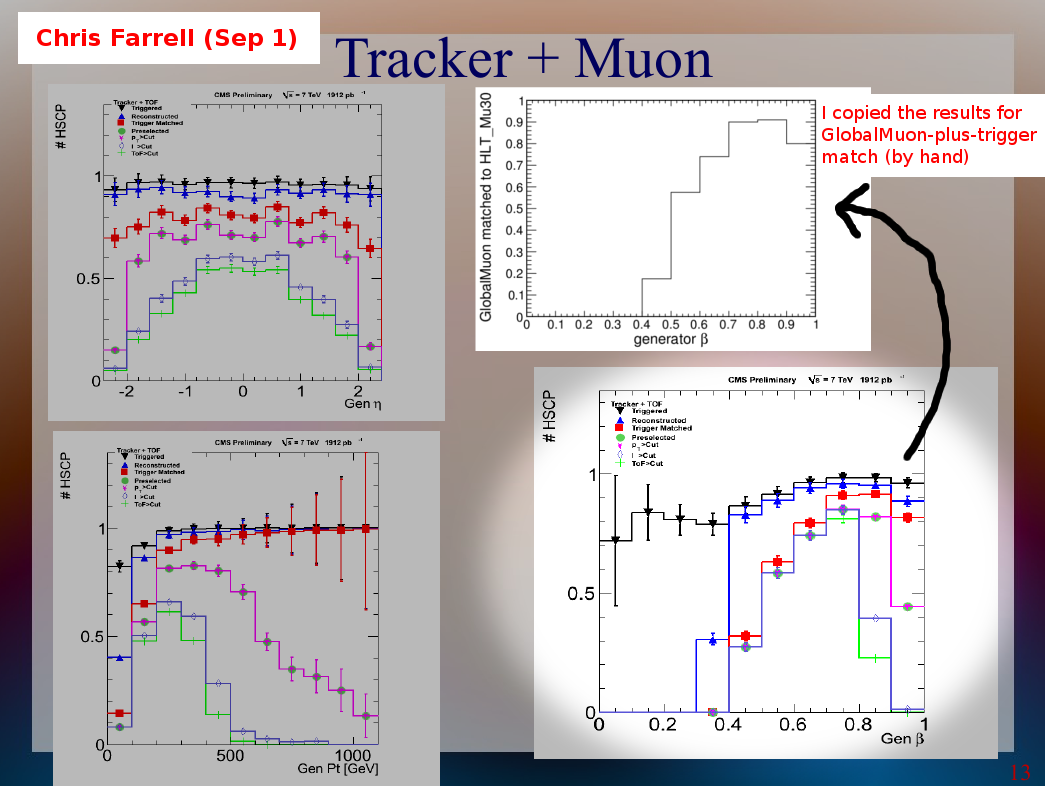
\includegraphics[width=0.9\linewidth]{originslide.png}
\end{center}
\end{frame}

\begin{frame}
\frametitle{Cross-section times acceptance vs.\ $\beta$}

\begin{itemize}
\item Raw distributions (no cuts) peak at high $\beta$, but most of these events are beyond the muon system and tracker in $\eta$
\item Requiring $|\eta| < 2.4$ shifts the distribution to low $\beta$, particularly for 250~GeV/$c^2$ quirks (right)
\item Muon trigger $\beta$ dependence applied by multiplying each bin with the plot from the previous page (assuming flat $\eta$ dependence)
\item It looks like we're losing a lot of $\beta < 0.5$ events to the muon trigger (though we still have 1~fb left for the 250~GeV/$c^2$ quirks)
\end{itemize}

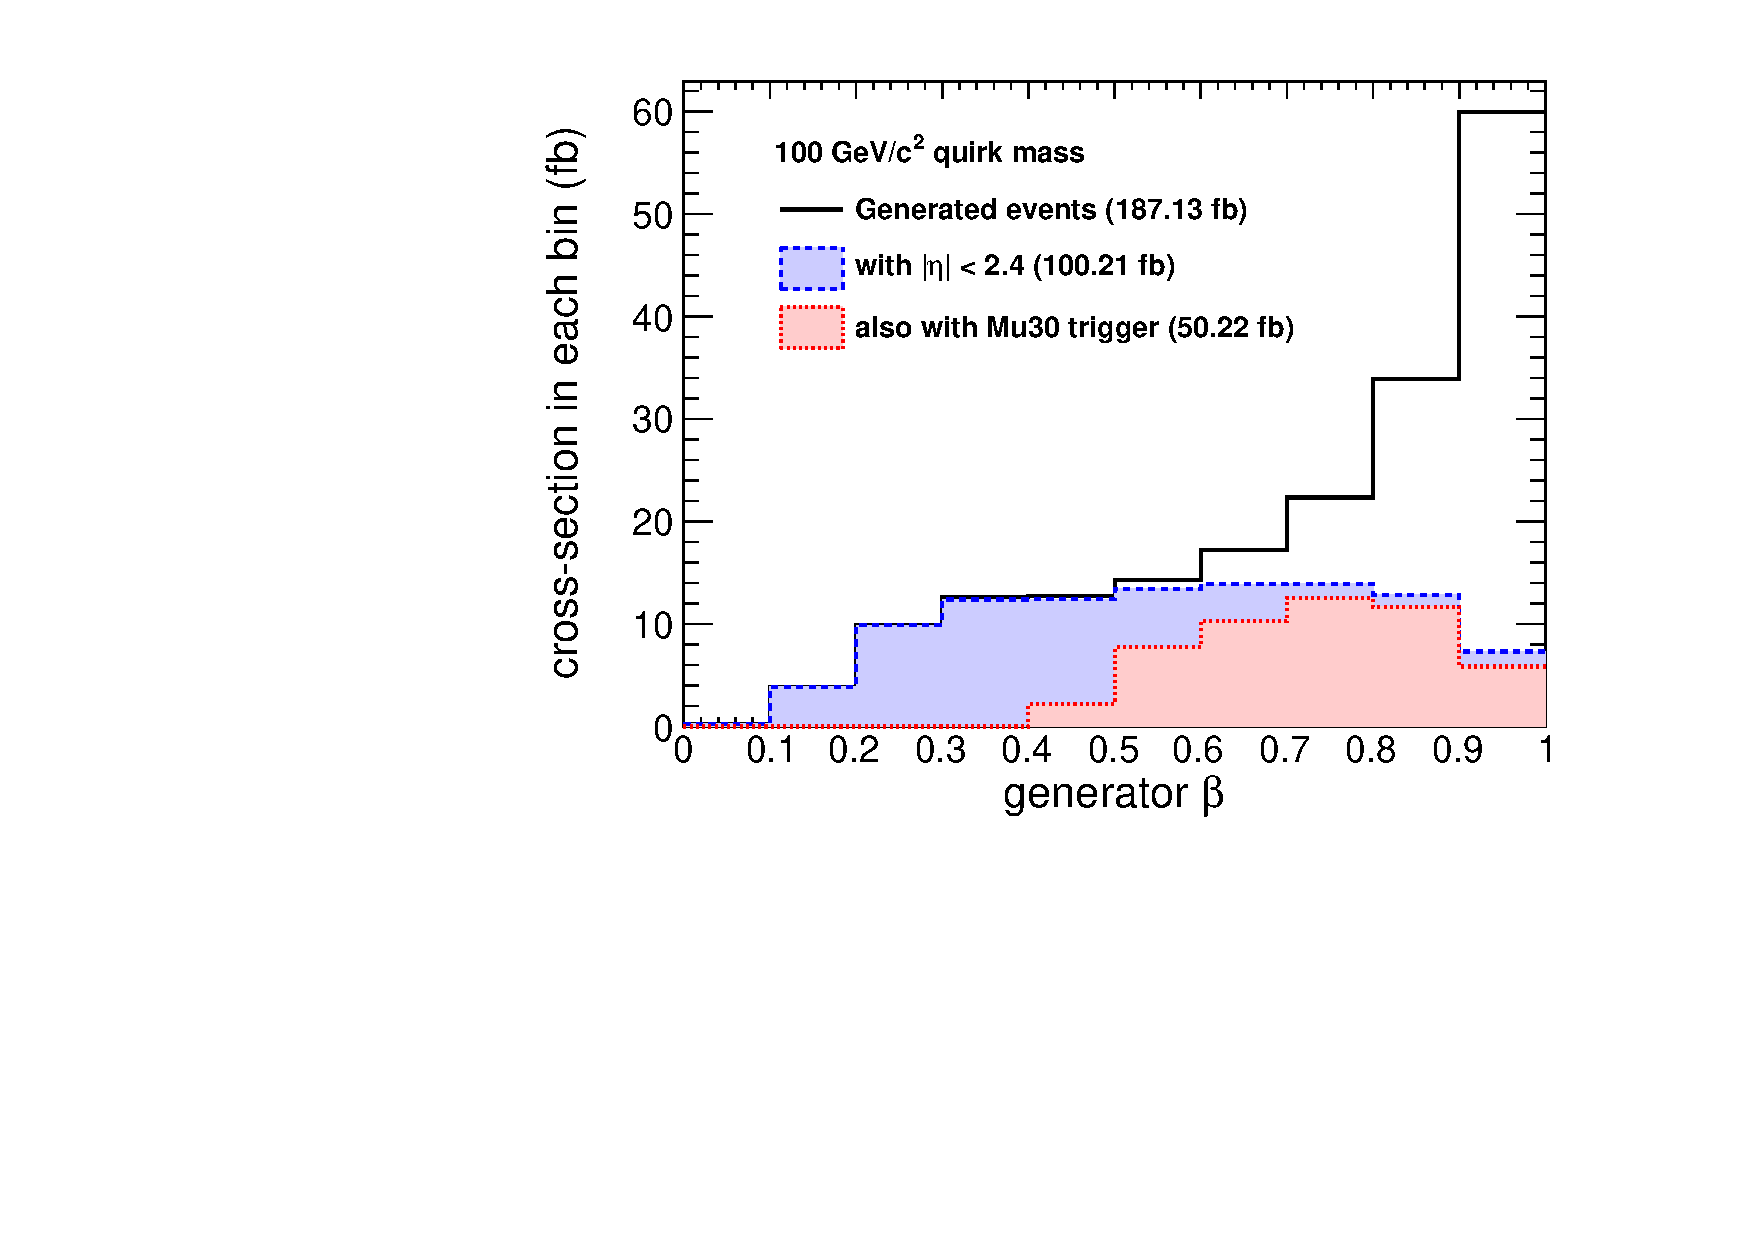
\includegraphics[width=0.5\linewidth]{mutrigger_100gev.pdf}
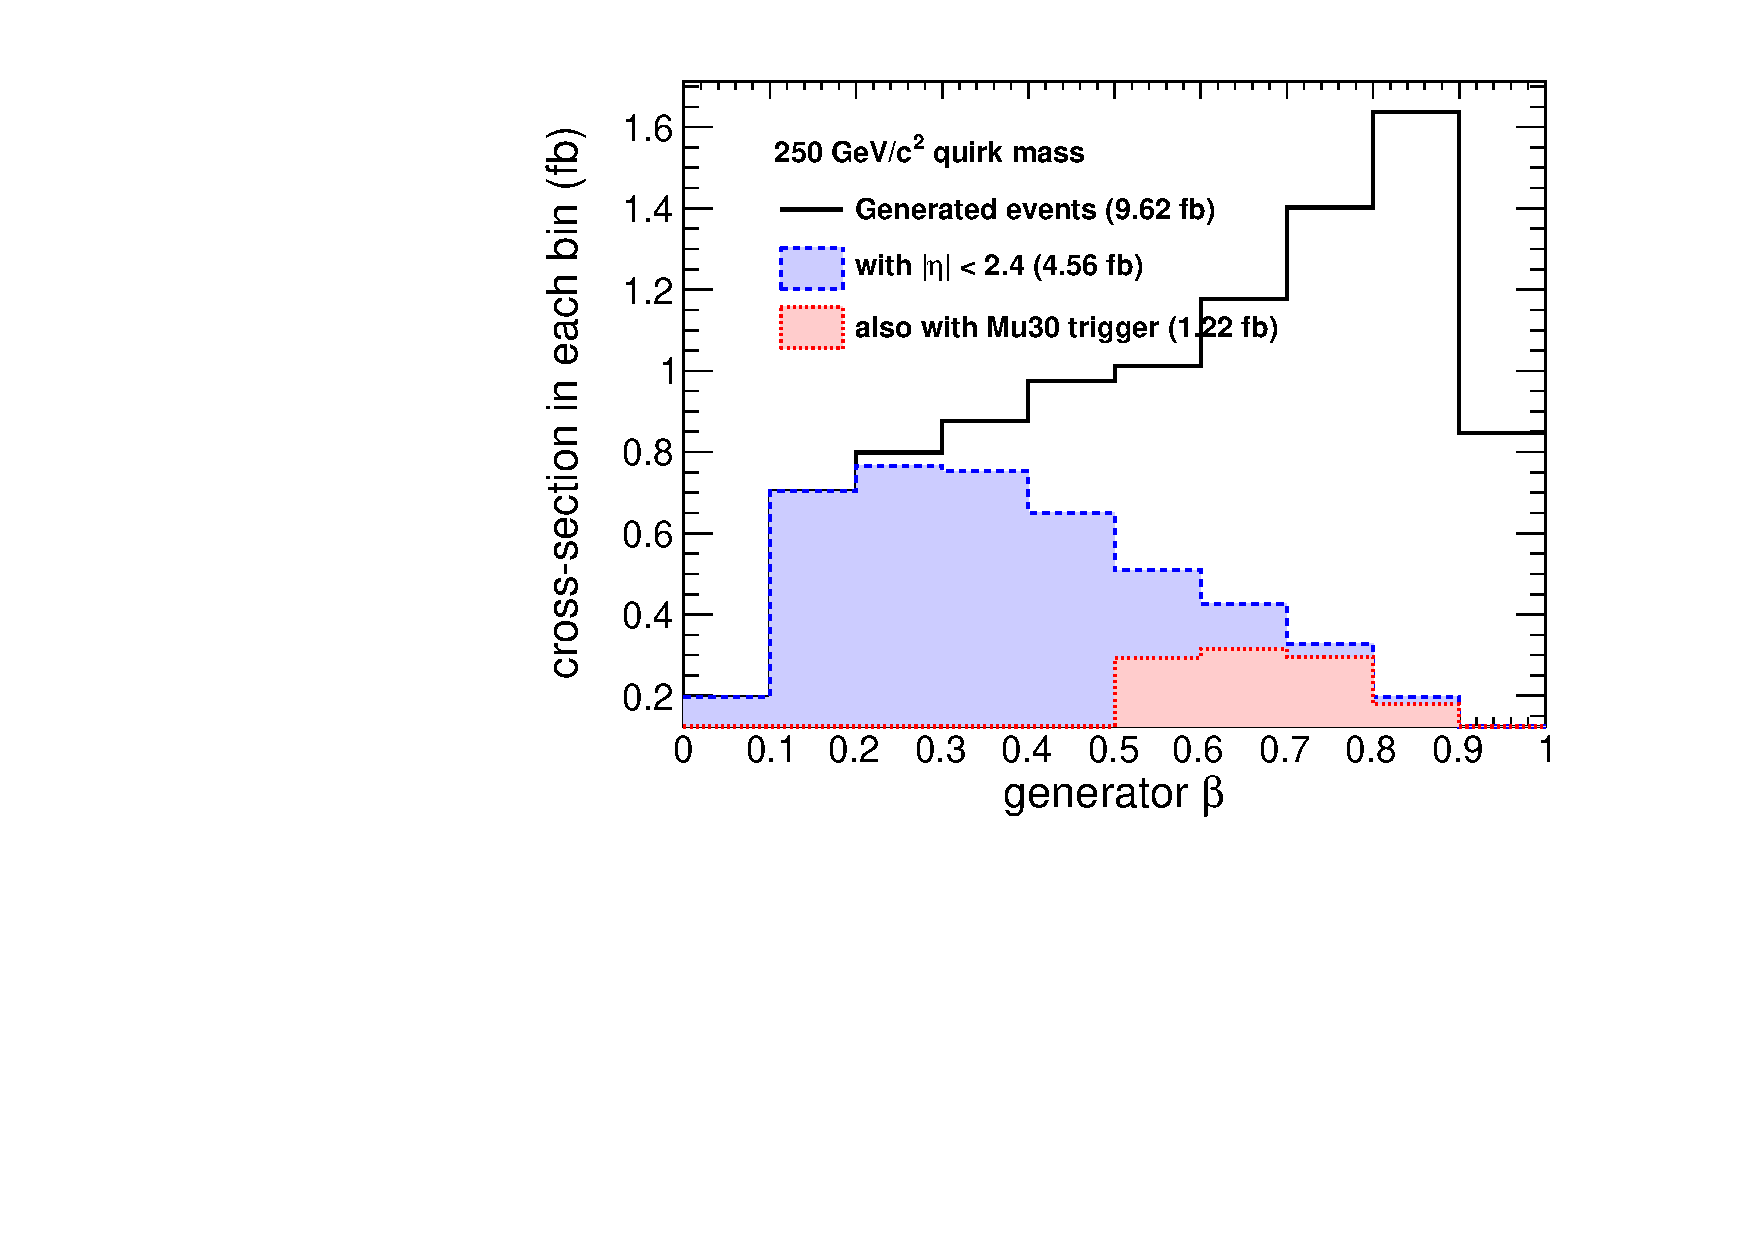
\includegraphics[width=0.5\linewidth]{mutrigger_250gev.pdf}
\end{frame}

\begin{frame}
\frametitle{Why the strong correlations among cuts?}

Kinematics: $\beta$ has an S-shaped dependence on $\eta$ because $p_T$ is nearly flat versus $\eta$ (with little dependence on quirk-pair mass)

\begin{center}
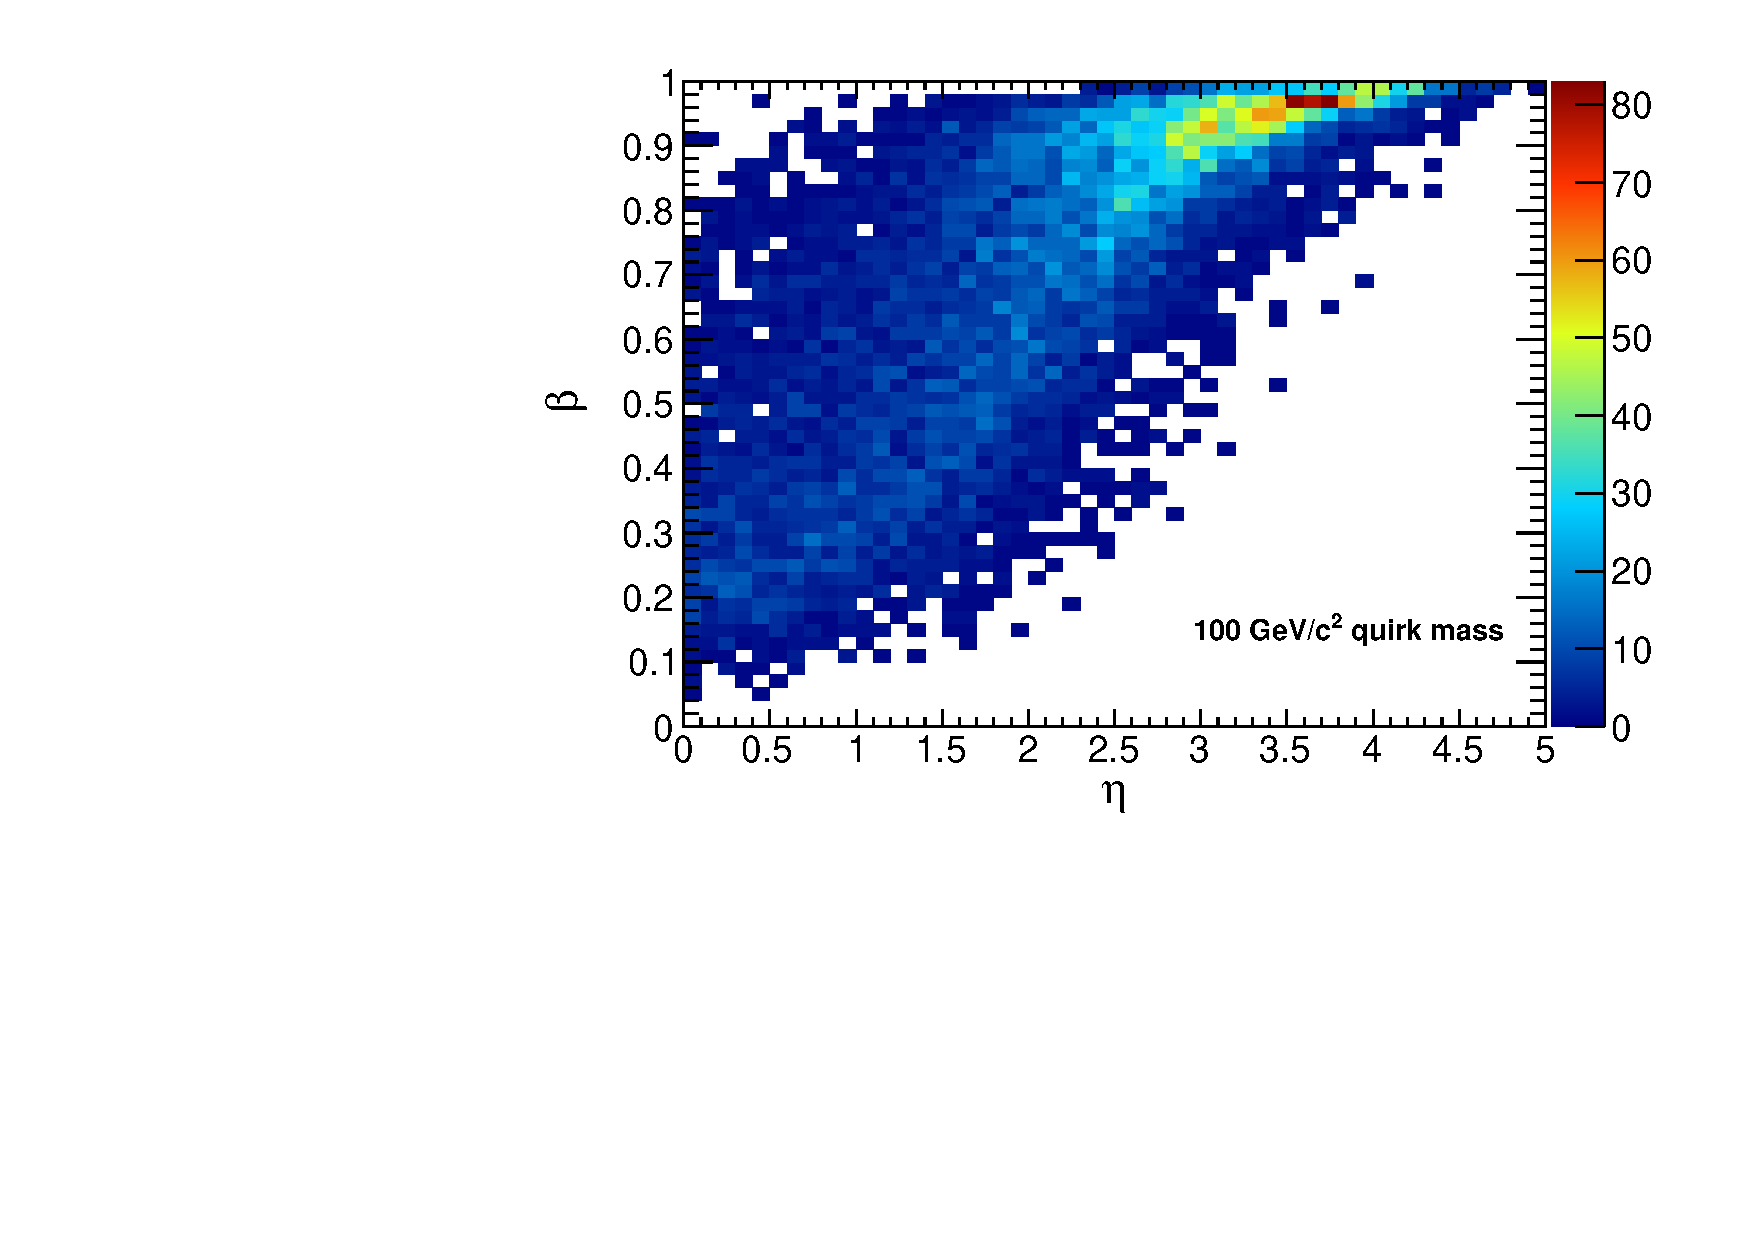
\includegraphics[width=0.5\linewidth]{why_100gev.pdf}
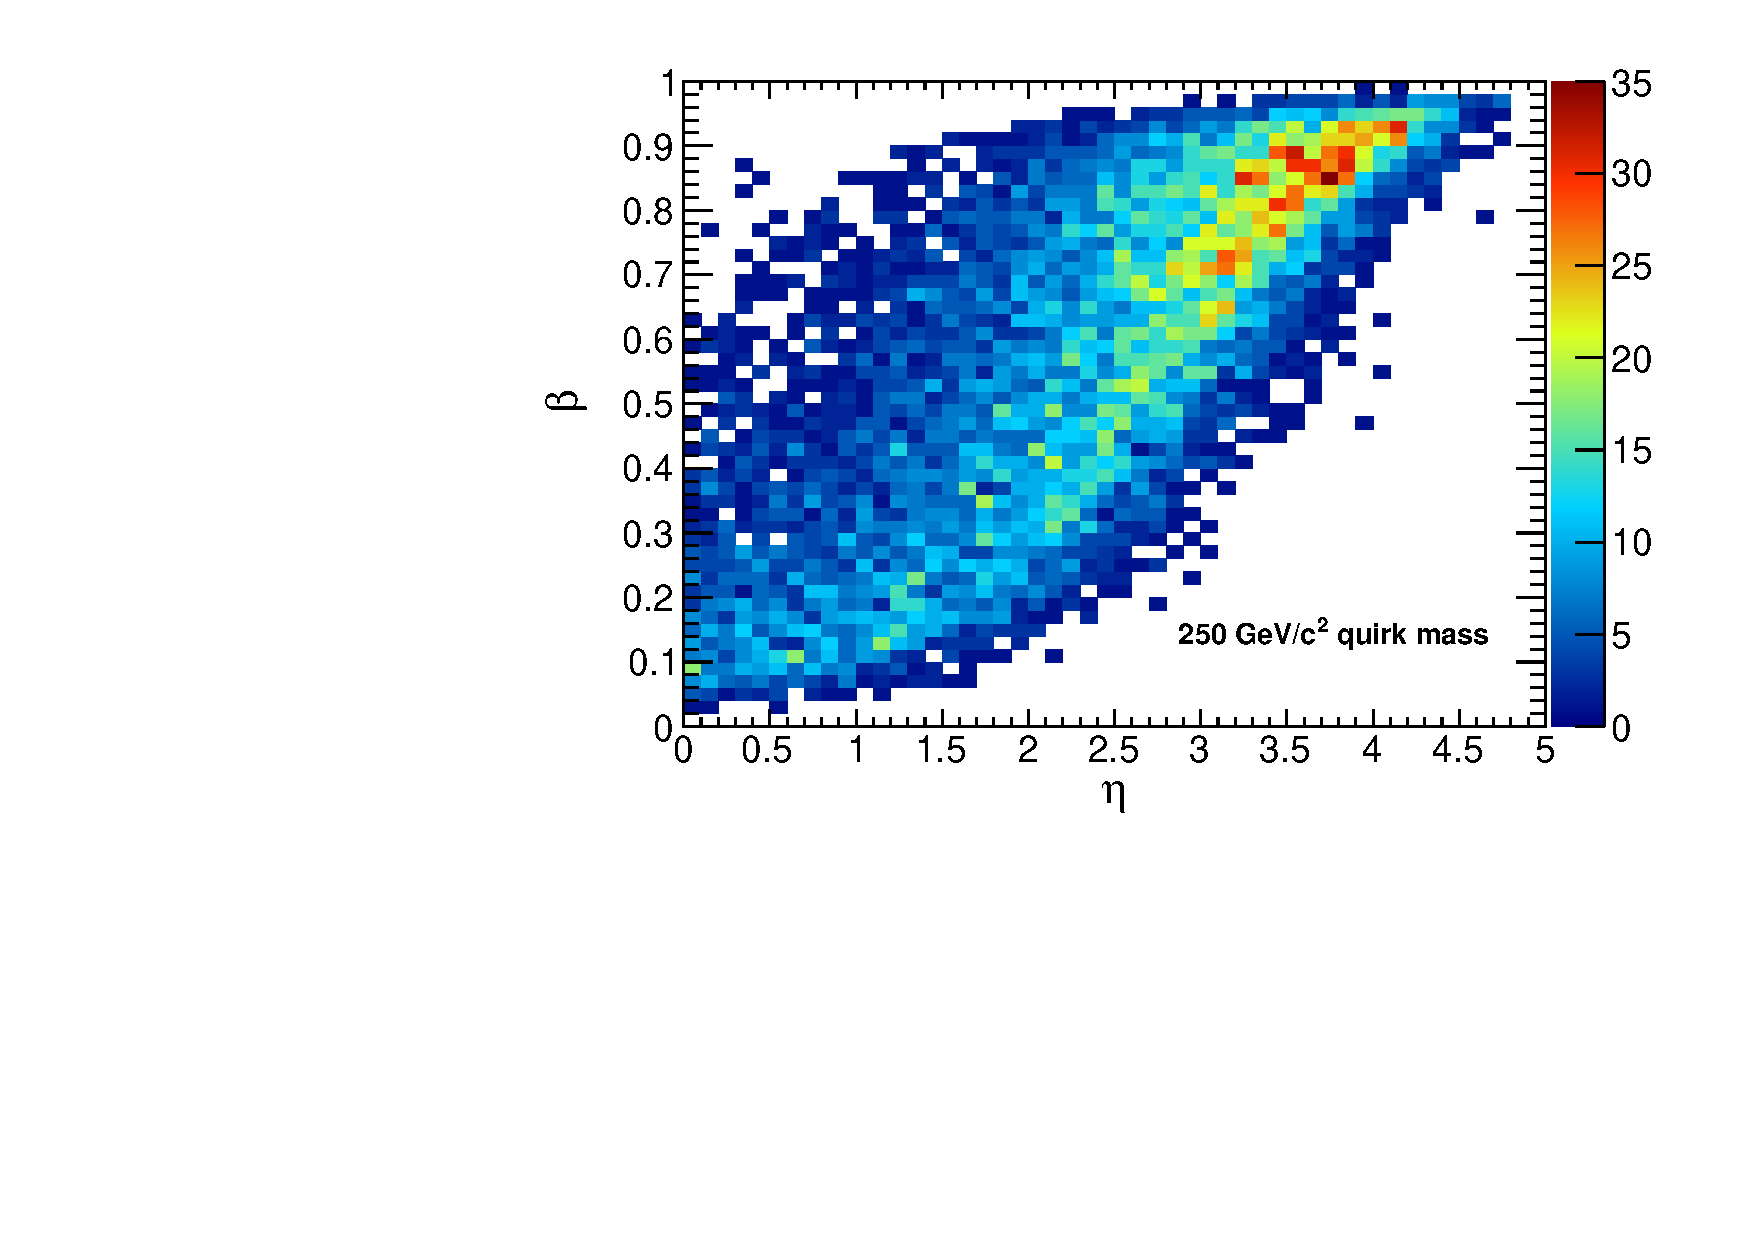
\includegraphics[width=0.5\linewidth]{why_250gev.pdf}

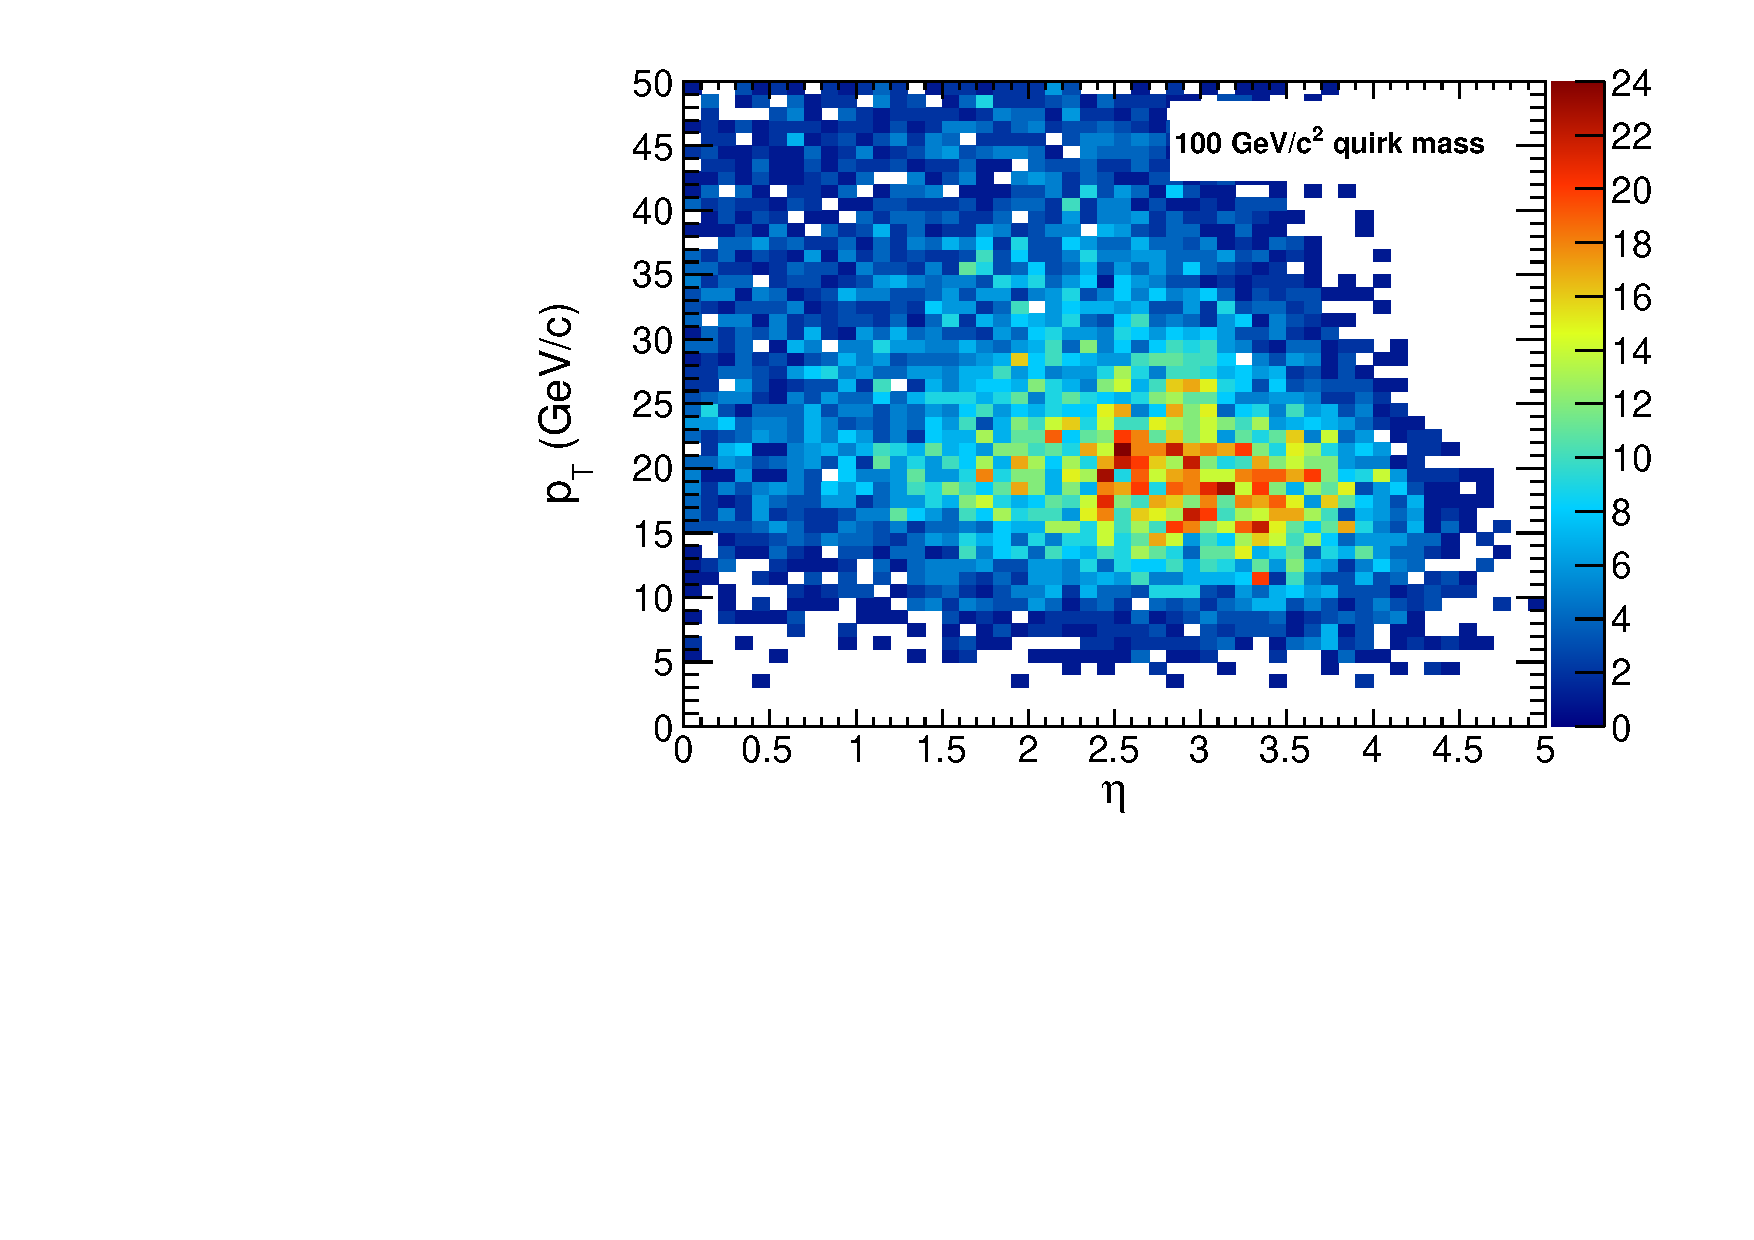
\includegraphics[width=0.5\linewidth]{why2_100gev.pdf}
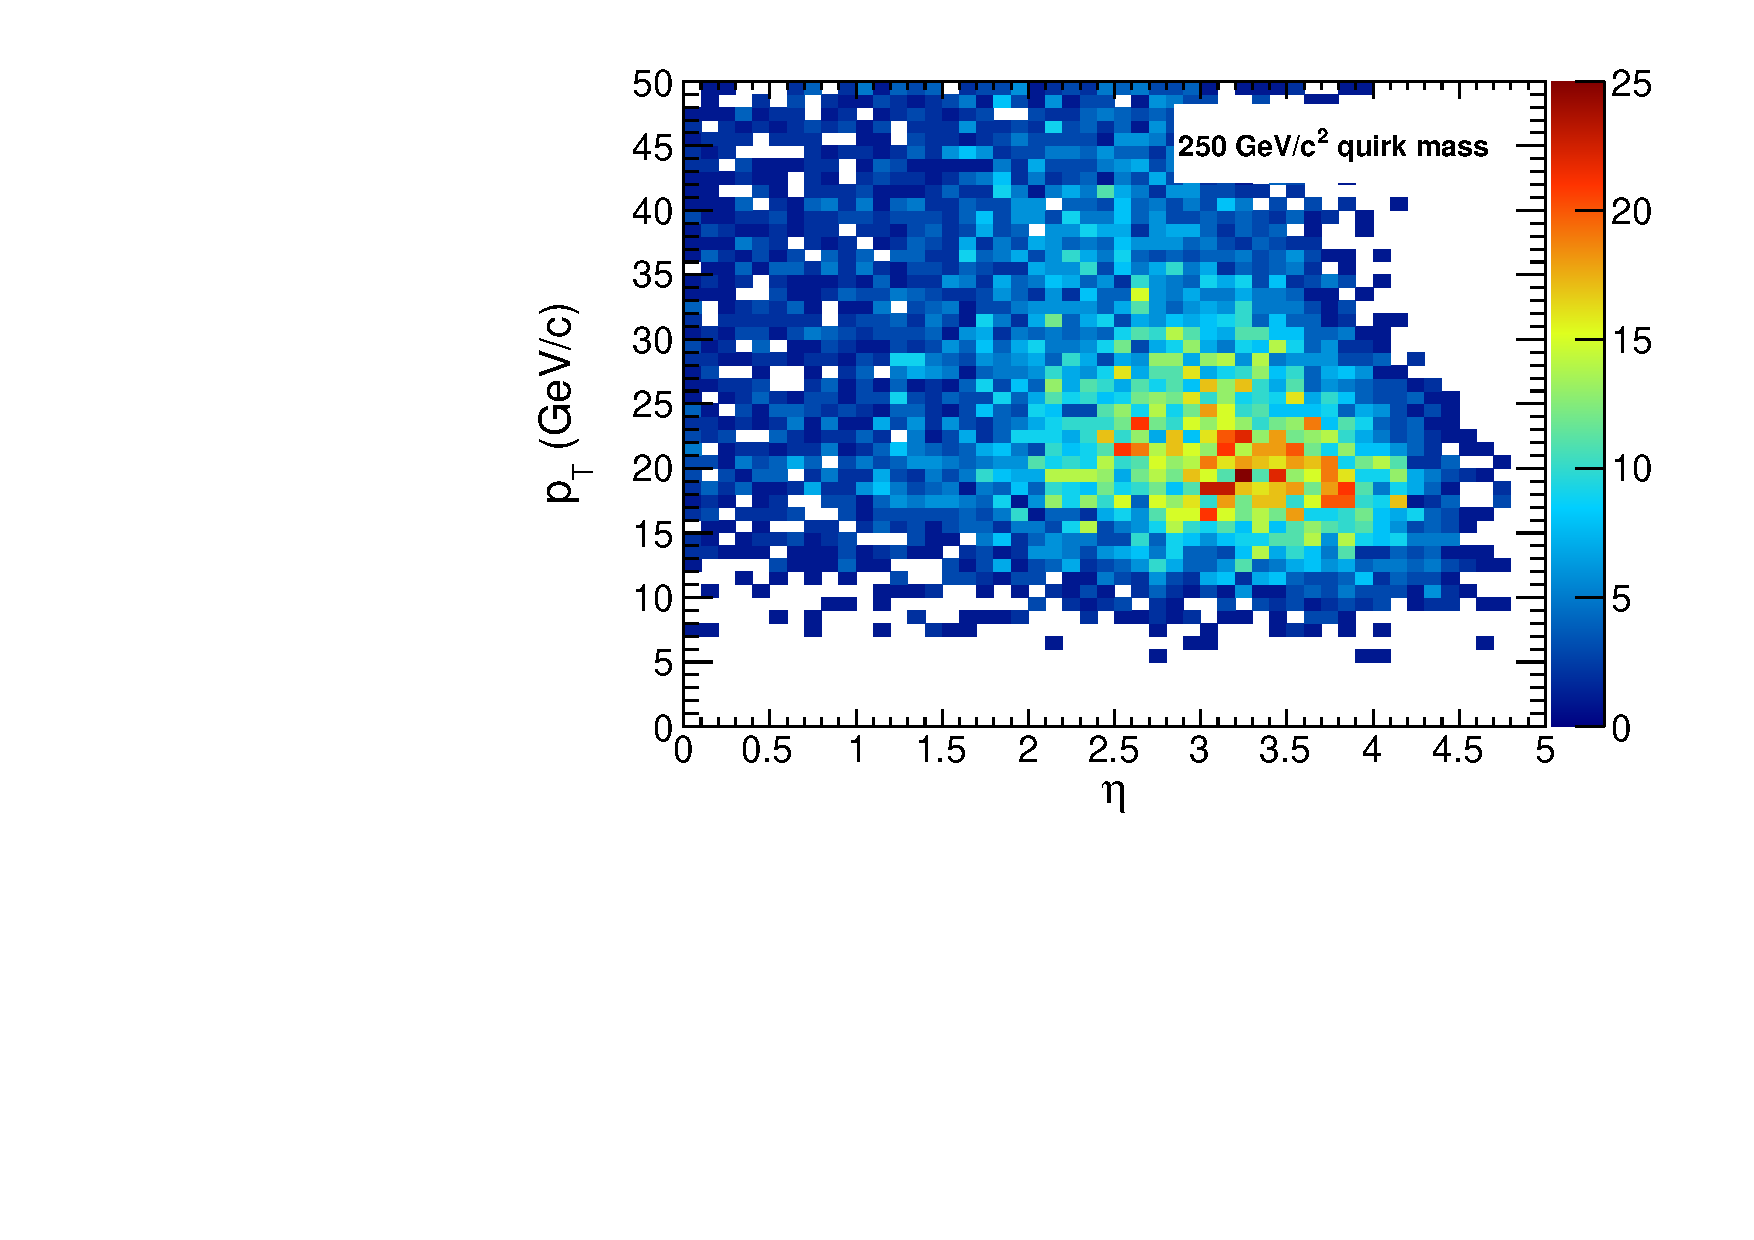
\includegraphics[width=0.5\linewidth]{why2_250gev.pdf}
\end{center}
\end{frame}

\begin{frame}
\frametitle{Could a jet trigger get the rest?}

Here are distributions of the ISR jet $p_T$ associated with the quirk-pair:

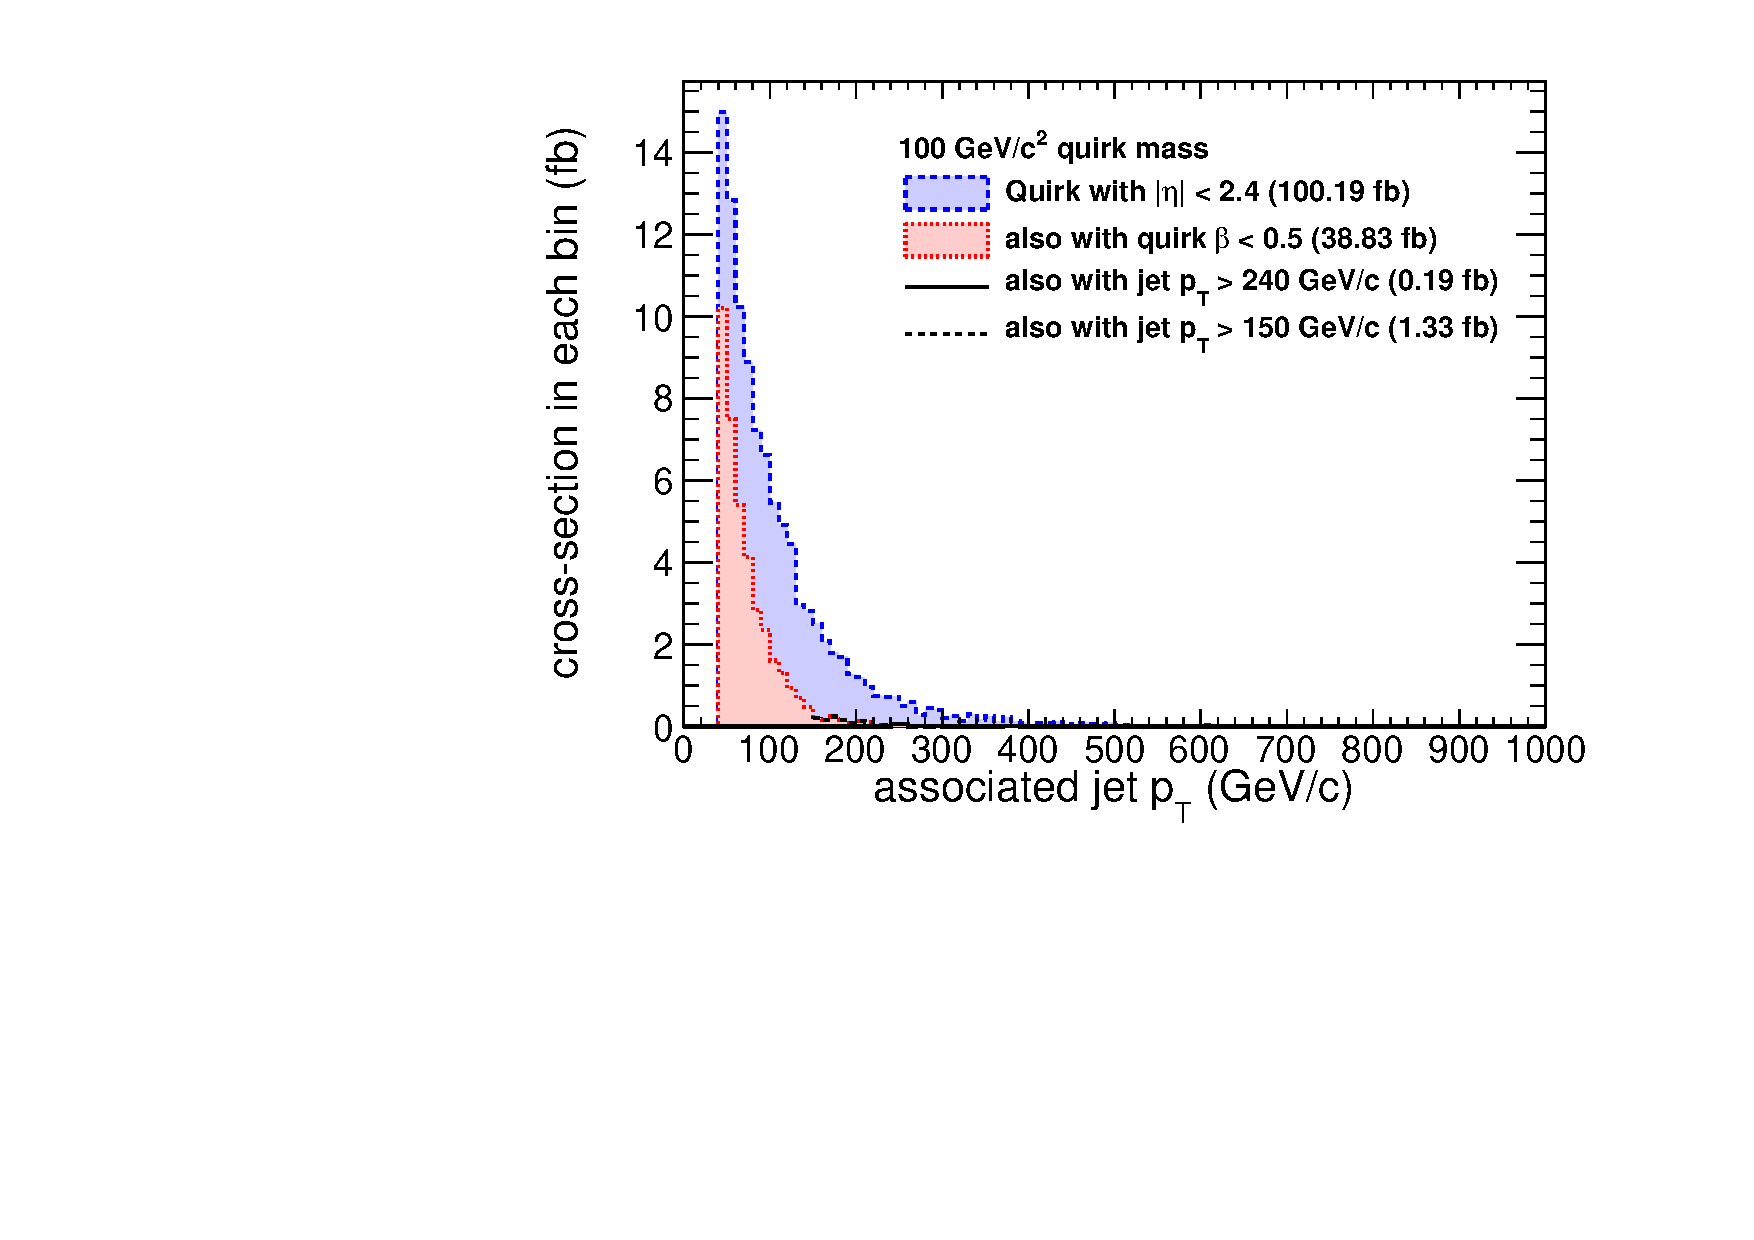
\includegraphics[width=0.5\linewidth]{jettrigger_100gev.pdf}
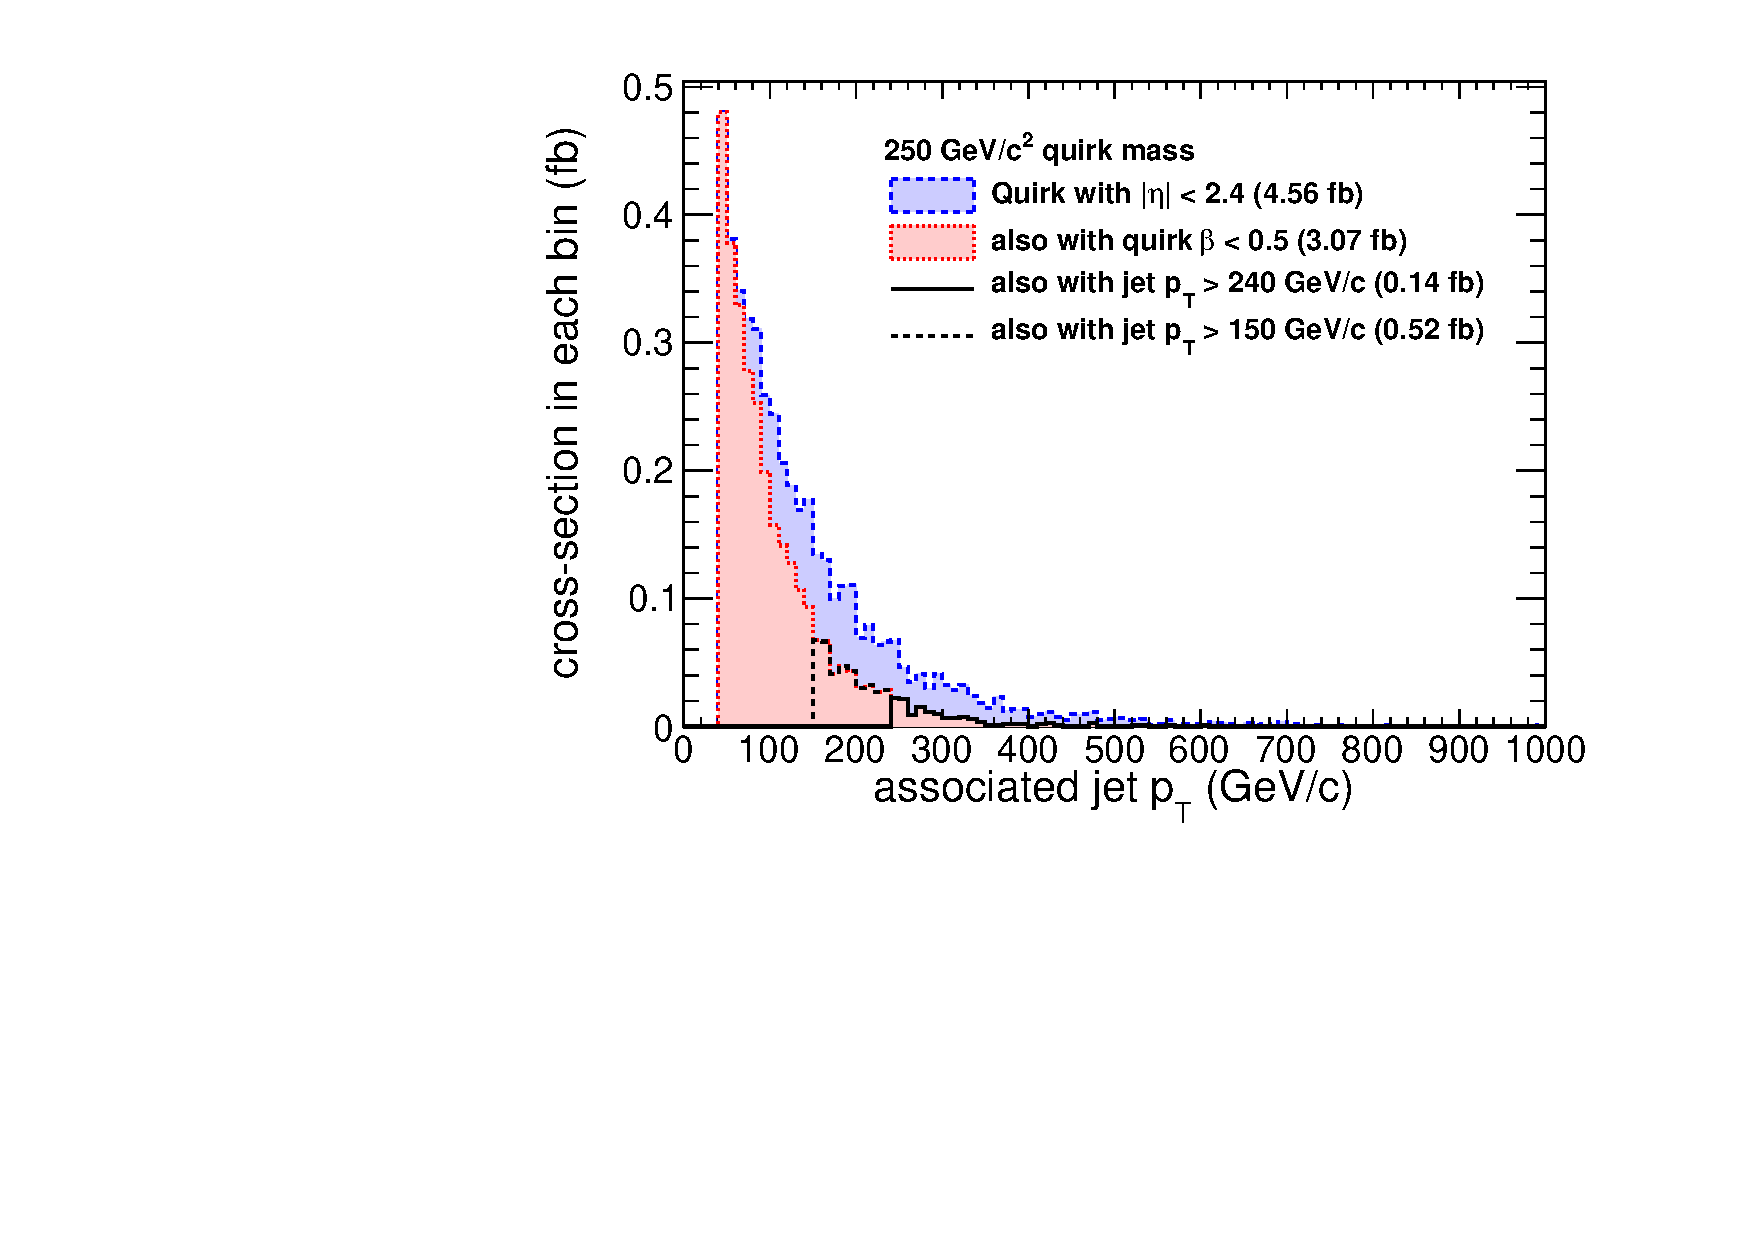
\includegraphics[width=0.5\linewidth]{jettrigger_250gev.pdf}

If the first unprescaled jet trigger is $p_T > 240$~GeV/$c$, or even $p_T > 150$~GeV/$c$, a jet trigger doesn't gain back much \textcolor{red}{(red is $\beta < 0.5$)}

\vspace{0.2 cm}
\hspace{-0.83 cm} \textcolor{darkblue}{\Large What about missing energy triggers?}

\vspace{0.1 cm}
The jet and the quirk-pair are back-to-back in these events (in $\phi$): \\ no invisible particles to give us real missing energy.

\vspace{0.2 cm}
\hspace{-0.83 cm} \textcolor{darkblue}{\Large Could the quirk-pair itself be fake missing energy?}

\vspace{0.1 cm}
Even if a no-tracking MET (e.g.\ CaloMET) considers the whole quirk-pair as missing energy, it only has $p_T \sim 20$~GeV/$c$ (prev page), not enough
\end{frame}

\begin{frame}
\frametitle{Estimated reach of muon-trigger-only}

\vspace{0.5 cm}
\renewcommand{\arraystretch}{1.2}
\begin{tabular}{l c c}
& 100 GeV/$c^2$ quirks & 250 GeV/$c^2$ \\\hline
Theoretical cross-section ($SU(2)$) & 187~fb & 9.6~fb \\
\ldots with $|\eta| < 2.4$ & 100~fb (53\%) & 4.6~fb (48\%) \\
\ldots matching Mu30 trigger & 50~fb (26\%) & 1.2~fb (13\%) \\
\ldots and $\beta < 0.8$ \mbox{(estimate of analysis cuts)\hspace{-0.8 cm}} & 33~fb (18\%) & 1.0~fb (10\%) \\
\textcolor{gray}{\ldots and $|\eta| < 2.0$ \mbox{(unnecessary preselection?)\hspace{-0.8 cm}}} & \textcolor{gray}{23~fb (12\%)} & \textcolor{gray}{0.60~fb (6\%)} \\\hline
Expected in 3~fb$^{-1}$ \mbox{(without preselection)\hspace{-0.8 cm}} & 99 & 3.0 \\
\end{tabular}

\begin{center}
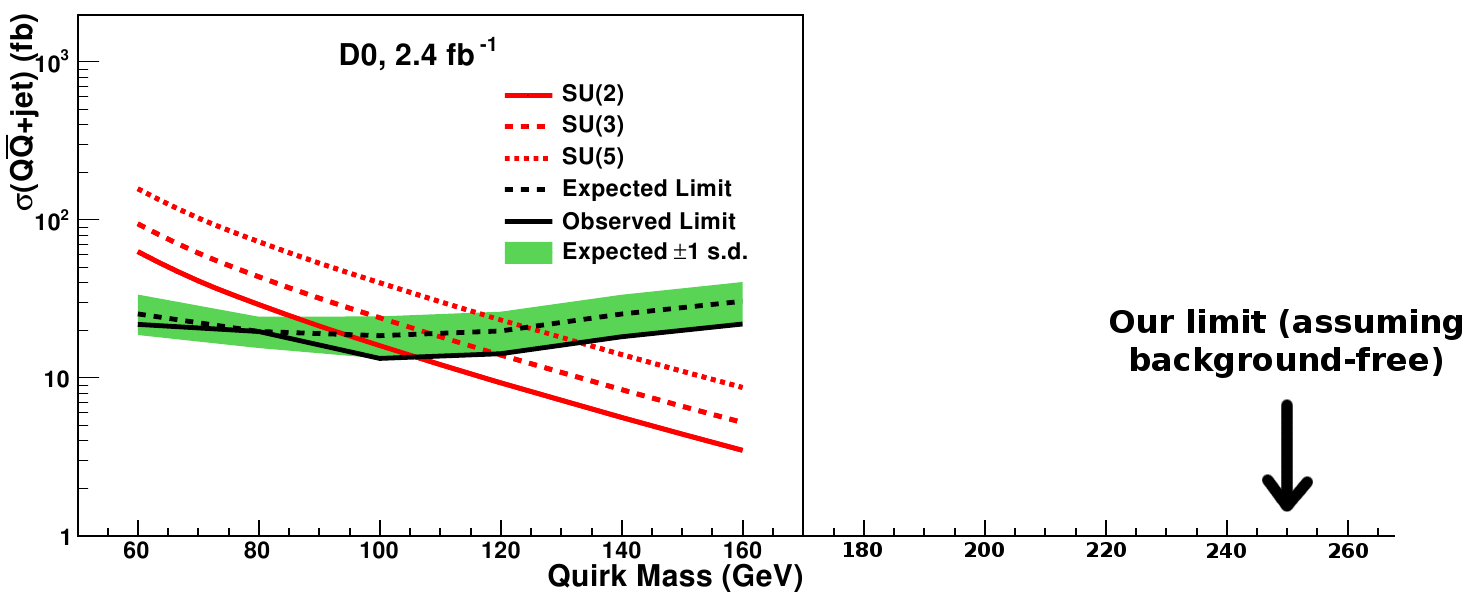
\includegraphics[width=0.9\linewidth]{d0_limit.png}
\end{center}
\end{frame}

%% \section*{First section}
%% \begin{frame}
%% \begin{center}
%% \Huge \textcolor{blue}{First section}
%% \end{center}
%% \end{frame}

\begin{frame}
\frametitle{Conclusions from this study}
\begin{itemize}
\item Using the muon trigger only would be a pretty good analysis
\item No other options are evident: jets (used by D\O) are significantly below our current thresholds (at least, one cannot buy back the muon trigger losses with jets)
\end{itemize}

\vspace{0.2 cm}
\hspace{-0.83 cm} \textcolor{darkblue}{\Large Other conclusions}

\vspace{0.1 cm}
\begin{itemize}
\item This model prefers high $\eta$: endcaps should be a particular focus
\item ``Preselection'' on Chris Farrell's slides has high, flat efficiency for $|\eta| < 2.0$, but very low efficiency outside of this range
\item Perhaps I should release the preselection cuts (since the curvature constraint provides other good handles): does this imply re-skimming?
\end{itemize}

\vspace{0.2 cm}
\hspace{-0.83 cm} \textcolor{darkblue}{\Large Next}

\vspace{0.1 cm}
\begin{itemize}
\item Get quirks into CMSSW \mbox{(Jie Chen has pointed me in the right direction)\hspace{-1 cm}}
\end{itemize}

\label{numpages}
\end{frame}

\end{document}
